%! Author = Romain
%! Date = 5/01/22

% Preamble
\documentclass[a4paper,11pt]{article}
\usepackage[english]{babel}
\title{Introduction à la cryptographie : Implémentation algo de chiffrement d'El Gamal}
\author{Romain Duc, Alexandre Serratore}
\date{6 mars 2023}

% Packages
% Symboles
\usepackage{amsmath}

% Graphes
\usepackage{pgf}
\usepackage{tikz}
\usetikzlibrary{positioning}

% Mise en page
\usepackage{multicol}
\usepackage{listings}
\usepackage{hyperref}

\usepackage{listings}
\usepackage{framed}

\lstset{
        language=Java,
        basicstyle=\ttfamily\small, %
        identifierstyle=\color{black}, %
        keywordstyle=\color{teal}, %
        numberstyle=\color{green},
        stringstyle=\color{black!64}, %
        commentstyle=\it\color{gray}, %
        columns=flexible, %
        tabsize=2, %
        extendedchars=true, %
        showspaces=false, %
        showstringspaces=false, %
        numbers=left, %
        numberstyle=\tiny, %
        breaklines=true, %
        breakautoindent=true, %
        captionpos=b,
        backgroundcolor=\color{lightgray!5},
        captionpos = b
}

% Document
\begin{document}

        \maketitle
        \label{subsec:Q1}
        \textbf{Question 1 : \\}Quel langage de programmation avez-vous choisi ? Quelle bibliothèque permettant de gérer des nombres entiers de grande taille allez-vous utiliser ? Quelles sont les opérations implémentées dans cette bibliothèque (multiplication, addition,...) ?\\ \textit{\\Réponse :} \\Nous avons choisi d'utiliser le langage Java. Java nous a paru l'option la plus adaptée, car il dispose de bibliothèques mathématiques intégrées permettant d'effectuer des opérations complexes, e.g. l'exponentiation modulaire.\\La classe\textit{ java.math.BigInteger } permet de représenter et de manipuler des nombres entiers de grande taille sans être contraint par les limitations de taille des types primitifs ou leurs enveloppes. Il est possible d'utiliser cette classe pour effectuer des soustractions, des modulos, des multiplications. En plus des opérations habituelles sur les entiers, elle offre des opérations de calcul en arithmétique modulaire, calcul du pgcd, génération de nombre premier, test pour savoir si un entier est premier, etc...  \\\\

        \label{subsec:Q2}
        \textbf{Question 2 : \\}De plus, pour générer les valeurs (très grandes elles aussi), $x$ et $r$, il faut être capable de générer des nombres aléatoires de très bonne qualité et dits cryptographiquement sûrs.\\En vous aidant d’internet, donnez la définition d’un nombre aléatoire cryptographiquement sûr. Selon le langage de programmation choisi, donnez le nom de la bibliothèque qui va vous permettre de générer ces nombres aléatoires.\\ \textit{\\Réponse :}\\\\Un nombre aléatoire cryptographiquement sûr est un nombre:\\ - Généré aléatoirement qui est difficile à prédire ou à reproduire, même en utilisant les informations sur la façon dont il a été généré\\ - Aléatoire indépendant des autres nombres aléatoires générés précédemment.\\ - Très difficile, étant donné les $k$ premiers bits d'une séquence, de trouver le $(k+1)$-ème bit à l'aide d'un algorithme polynomial avec un taux de succès de plus de 50\%.\\ Ces nombres sont souvent utilisés pour sécuriser les communications cryptographiques en générant des clés de chiffrement ou en ajoutant du bruit à des communications pour empêcher qu'elles ne soient déchiffrées.\\
        Nous utiliserons la bibliothèque "SecureRandom" de Java pour générer des nombres aléatoires cryptographiquement sûrs. Voici une exemple d'utilisation de cette bibliothèque:\\\\ \begin{lstlisting}
import java.security.SecureRandom;

SecureRandom random = new SecureRandom().getInstanceStrong();
int randomInt = random.nextInt();

        \end{lstlisting}
        \begin{itemize}
                \item \url{https://miashs-www.u-ga.fr/prevert/Prog/Java/CoursJava/lesBig.html}
                \item \url{https://stackoverflow.com/questions/11051205/difference-between-java-util-random-and-java-security-securerandom}
        \end{itemize}

        \textbf{\\Question 3 : \\}Implémentez la fonction Euclide(). Testez là en vérifiant sur 10000 valeurs différentes de a que a · u + p · v = 1. Vous pouvez également vérifier que si une fonction existe déjà dans votre librairie, vous retournez bien les mêmes valeurs.
        \textit{\\Réponse :} \\\\Nous avons implémenté la fonction Euclide() en utilisant l'algorithme d'Euclide étendu (solution itérative). Cette fonction prends donc en paramètre 2 \textit{BigInteger} puis retourne un tableau de \textit{BigInteger} contenant PGCD(a,b) ainsi que les coefficient u et v aux indices respectifs [0], [1] et [2].\\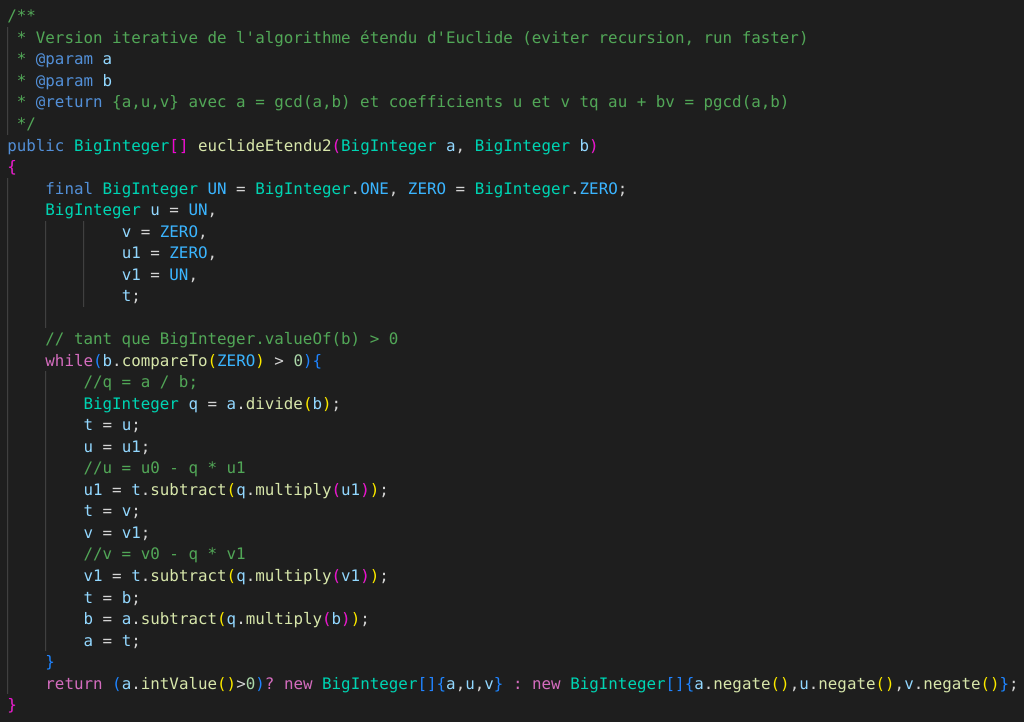
\includegraphics[scale=0.4]{assets/euclide.png}\\Nous avons testé cette implémentation à l'aide de la fonction \textit{ void test10000Times(BigInteger p, SecureRandom random) } (Voir ci-après).\\Pour le même entier \textit{p} nous générons 10000 valeurs de \textit{a} à l'aide de SecureRandom et nous appellons la fonction Euclide() définie précédement. Puis nous vérifions à l'aide de 3 assert que:\\ - le tableau retourné contient bien le gcd(a,p) (A l'aide de la fonction \textit{gcd(p)} de la classe \textit{BigInteger})\\ - le gcd(a,p) est bien égale à au + pv\\ - l'équation de bezout donne bien 1\\\\ Nous affichons les 5 derniers résultat dans le fichier "test.txt". \\\\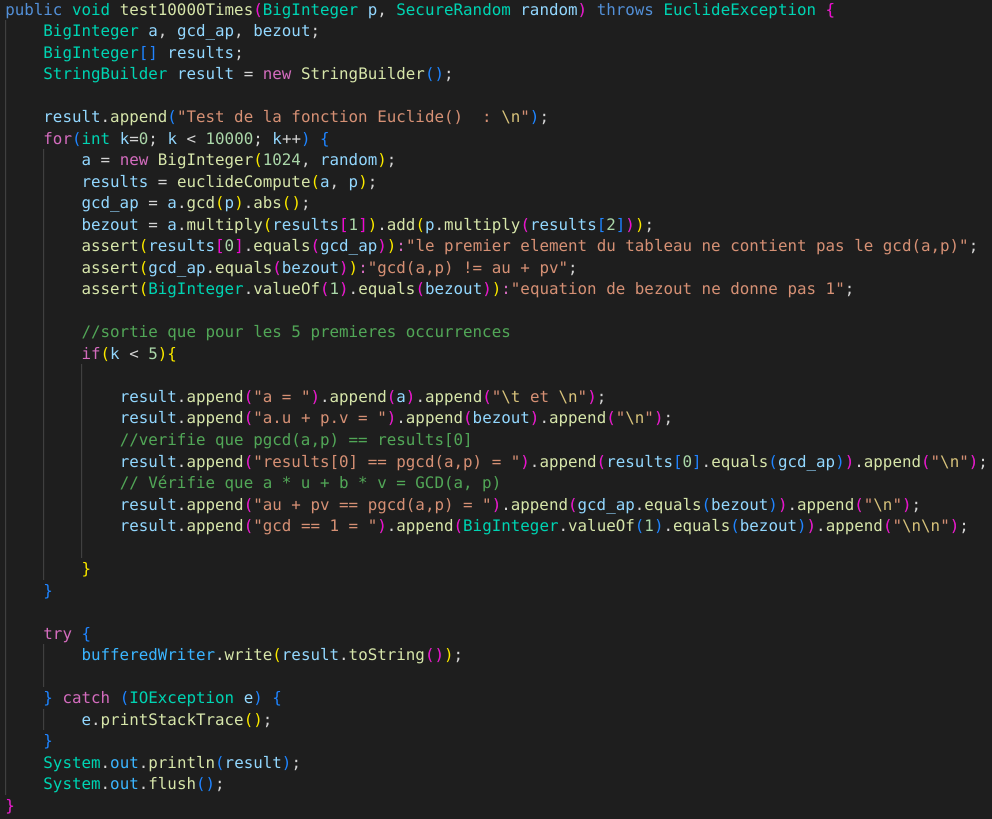
\includegraphics[scale=0.3]{assets/testEucl.png}


        \textbf{\\Question 4 : \\}Implémentez la fonction ExpMod(). Testez-la sur 10000 valeurs différentes.
        \textit{\\Réponse :} \\\\Nous avons implémenté cette fonction en utilisant l'algorithme de l'exponentiation rapide avec \textit{ BigInteger expMod(BigInteger p, BigInteger g, BigInteger a) } qui se situe dans la classe \textit{ExponentiationModulaire.java}. Cette fonction prends donc en paramètre 3 \textit{BigInteger} puis retourne un  \textit{ BigInteger A = $(g^a \equiv p)$} . \\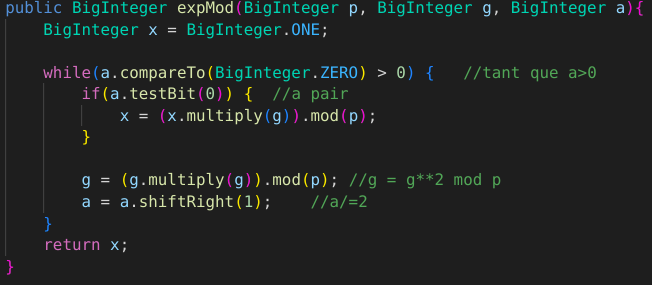
\includegraphics[scale=0.4]{assets/ExpMod.png}\\Nous avons testé cette implémentation à l'aide de la fonction \textit{ void test10000Times(BigInteger p, BigInteger g, SecureRandom sr) (Voir ci-après}.\\Pour le même entier \textit{p} nous générons 10000 valeurs de \textit{a} à l'aide de SecureRandom et nous appellons la fonction Euclide() définie précédement. Puis nous vérifions à l'aide de 3 assert que:\\ - le tableau retourné contient bien le gcd(a,p) (A l'aide de la fonction \textit{gcd(p)} de la classe \textit{BigInteger})\\ - le gcd(a,p) est bien égale à au + pv\\ - l'équation de bezout donne bien 1\\ Nous affichons les 5 derniers résultat dans le fichier "test.txt". \\\\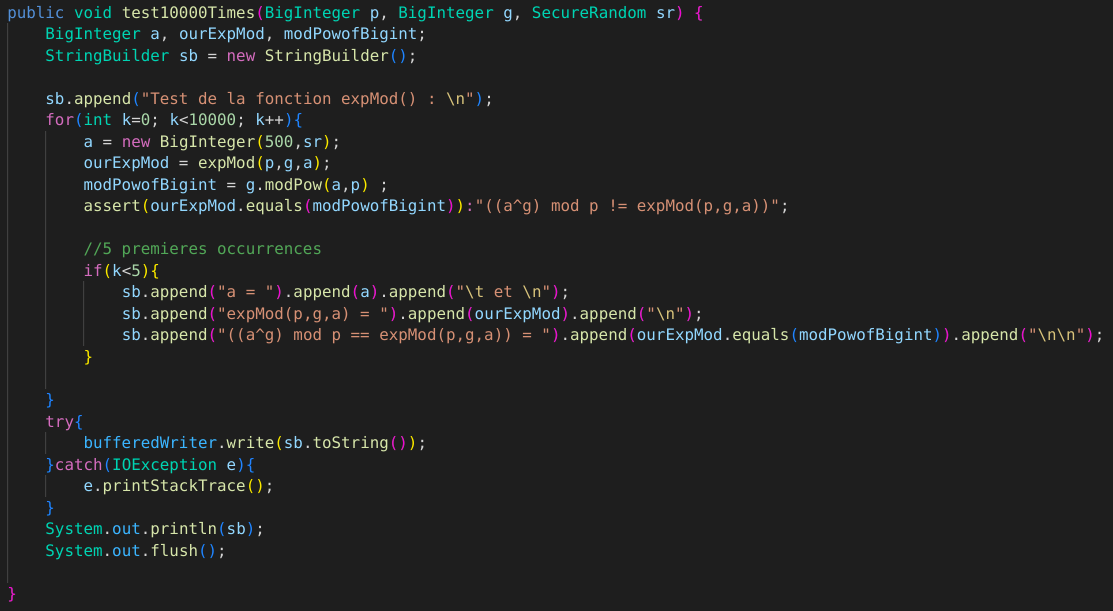
\includegraphics[scale=0.3]{assets/testExpMod.png}


        \textbf{\\Question 5 : \\}Implémentez ces trois fonctions. Testez-la en vérifiant que 100 valeurs différentes de m donne bien les déchiffrés attendus (c’est-à-dire de nouveau les m!). Vérifiez également que les 100 r tirés au hasard sont bien différents.
        \textit{\\Réponse :} \\\\Nous avons implémenté les fonctions Encrypt(), Decrypt().\\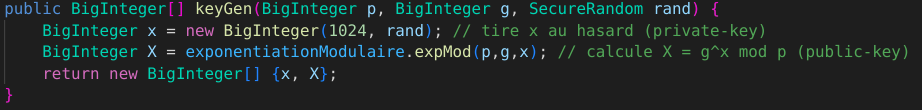
\includegraphics[scale=0.45]{assets/keygenEG.png}\\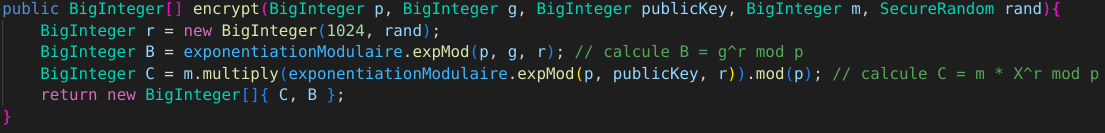
\includegraphics[scale=0.42]{assets/encryptEG.png}\\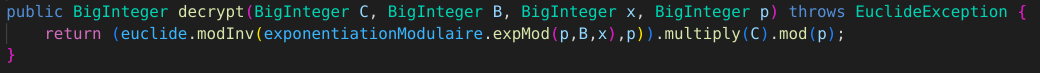
\includegraphics[scale=0.4]{assets/decryptEG.png} \\\\Voir la fonction de test ci-dessous : \\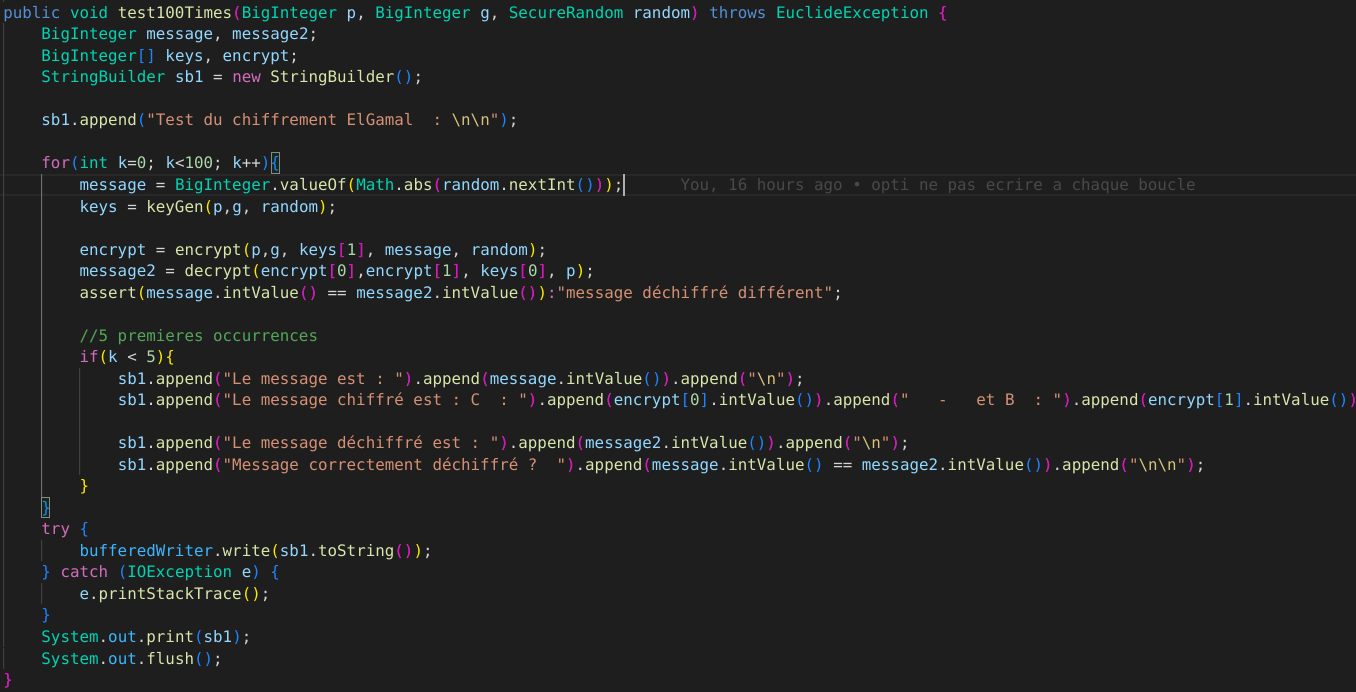
\includegraphics[scale=0.3]{assets/testElgamal.png}
        \\\\Nous avons également implanté une fonction permettant de calculer l'inverse modulaire d'un nombre. (utilisée dans la fonction Decrypt()) \\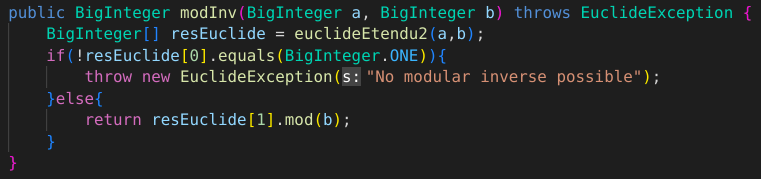
\includegraphics[scale=0.45]{assets/invMod.png}\\


        \textbf{\\Question 6 : \\}Vérifiez cette propriété en chiffrant deux messages différents m1 et m2 avec la fonction Encrypt(), puis en calculant C = C1 . C2 mod p et B = B1 . B2 mod p et enfin en déchiffrant via la fonction Decrypt() le couple (C, B) pour récupérer m. Vérifier ensuite que m = m1.m2 mod p.
        \textit{\\Réponse :} \\\\Nous avons implémenté la fonction de test ci-dessous qui test 5 fois la propriété : \\\\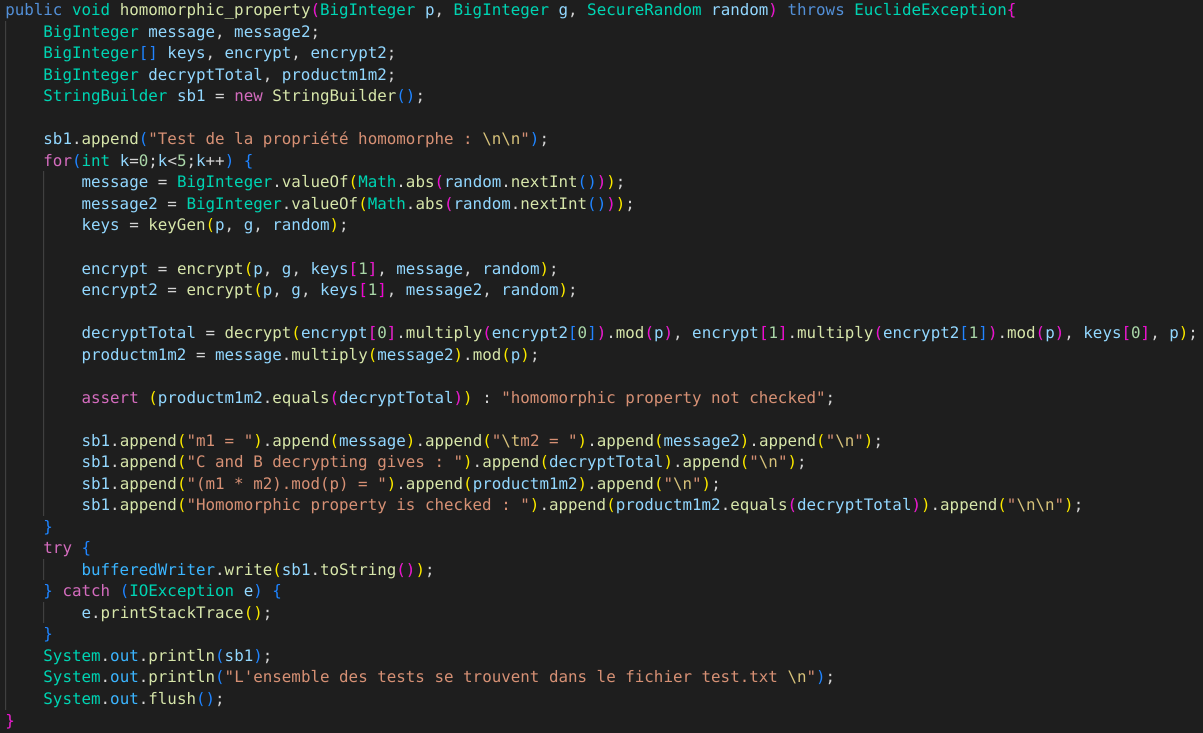
\includegraphics[scale=0.3]{assets/homo_prop.png}\\\\\\\


        \textbf{\\Fichier test.txt : }

        \begin{lstlisting}[caption ={le fichier test.txt}, captionpos=b,breaklines = true]
Test de la fonction Euclide()  : 
a = 160673951202871820768522432264413824281379564922918785062825317898190593802109840755896761432932396921370717923680995368632651713753124593343418110386158594003109874457006794327810034901124362304868722224106716023601094727602631269317995249471403818877294271903566082226945015280819860534613810788669181142655 et
a.u + p.v = 1
results[0] == pgcd(a,p) = true
au + pv == pgcd(a,p) = true
gcd == 1 = true

a = 178692563691092062429232399272601670879140757709494040679319707602107499034757832117396622593819258118576208765751340049391086793819262707001263576304316965882916898524551880613703248267995736142789373890193765303933296483895225177716470098681267538381459571544678597351156562100160694233453703372198074925403 et 
a.u + p.v = 1
results[0] == pgcd(a,p) = true
au + pv == pgcd(a,p) = true
gcd == 1 = true

a = 178686959315835014564667448615041465056097822529956931805211106178921228239734109306721901497944637150575015899831448974892426985045808388703911684127372064587777485170648551837829545664940655151294550883657639048804958903374346976533090451645223528400958169203505829829473353815946210930698647261455270391978 et 
a.u + p.v = 1
results[0] == pgcd(a,p) = true
au + pv == pgcd(a,p) = true
gcd == 1 = true

a = 157964703148738141022575258235549864420432938373980654168295926249857798008255841642664404511207317166809777481697855997641388257161389902718534687620438268328893365738747403425492858594821889372685442418247611565157649550720632350481246844976845544125093251202712563018590019711332515298045258381423755311035 et 
a.u + p.v = 1
results[0] == pgcd(a,p) = true
au + pv == pgcd(a,p) = true
gcd == 1 = true

a = 132443799524215031501371190805309936511680265350275747540576235389840115523197368498347159308049620414822493485803422301906672653540803409802815944586910094455036396838045194706531559689821839601926836916226585504092800490455737561985281816791220438384614938447890176935510898070270806063376989730577414055179 et 
a.u + p.v = 1
results[0] == pgcd(a,p) = true
au + pv == pgcd(a,p) = true
gcd == 1 = true

Test de la fonction expMod() : 
a = 2548746397467316583521774692571175259635093069249366139817754030824443844383001006506780444082873915693407959776391867717161434678916643293256961828108 et 
expMod(p,g,a) = 8208755545454982530740916974116874655801127826989080145022266173067016516715817182174983183046473236864507043906801872058607908715503970307818477686703256748973957318540034983385303471678010146813073887016566115889074803406252798744886788720503484780554707969305456866240224561325426273798016633176640553319
((a^g) mod p == expMod(p,g,a)) = true

a = 2911721666508398710813225527311460356183275330200050706087490474229574356125601400286433689673648976682113519076116546990728567892911883730744836032866 et 
expMod(p,g,a) = 73363905545963107105003914753137274112973703659572693509760126773929094935829844726380238281309093186530128669524067723077801951294461794049554075950009525304224319047472103659964426734266884061857161595588354592776562499677063617200394774225886152922377012465339466363483488318418547461683462497070894366101
((a^g) mod p == expMod(p,g,a)) = true

a = 1385867912917292378582166082849174349562651642155716118173202440373363861834715048644196362636512435026694885936387442775085533955328675609162204638091 et 
expMod(p,g,a) = 59328179773782616061186709307340432600018969258278431480743255195732083346551391937584013989281787463633901874559741613021040096364124638994971632166408018359763218838571614139471612766920015049473941344039841499866235048814837671047879308346055141504993001414723084122012375505807920661433787716644657865145
((a^g) mod p == expMod(p,g,a)) = true

a = 3167678535301827418726468968822179013308680309635621093255789585371612781800649808464681152436007193128560042258983280356380582726410433892505442024172 et 
expMod(p,g,a) =  930889100551347572874547749083824538955126718317529216166615573332407299851481317412237094553042091849307227958113785550841195418634796980342523218043450354363610870550569321204965803046664052672475725160133953285904836428848177235627356724923320246192114030704715299649783615689390617958520014360354647413029
((a^g) mod p == expMod(p,g,a)) = true

a = 938569509273717994995711089912013032463309816207938245201274881809240462573981385057786855289849220819239038496022570535568318507009044288207030960259 et 
expMod(p,g,a) = 104665200528717005002774344799406697943664374101356463554085683117727154593081190744287800232340006945520367867992206439367910996834876882647232338414623590799173727253560108797757444763182337597920851105415078636410027809744672628114167544904014901912495642473794568658613636266577408682137832526948063896653
((a^g) mod p == expMod(p,g,a)) = true

Test du chiffrement ElGamal  : 

Le message est : 1369399431
Le message chiffre est : C  : 632760402   -   et B  : -1865444536
Le message dechiffre est : 1369399431
Message correctement dechiffre ?  true

Le message est : 1494697761
Le message chiffre est : C  : 2005268047   -   et B  : 155466468
Le message dechiffre est : 1494697761
Message correctement dechiffre ?  true

Le message est : 2125611792
Le message chiffre est : C  : -1588473933   -   et B  : -1907232047
Le message dechiffre est : 2125611792
Message correctement dechiffre ?  true

Le message est : 1308864376
Le message chiffre est : C  : 676242185   -   et B  : -663133218
Le message dechiffre est : 1308864376
Message correctement dechiffre ?  true

Le message est : 934934231
Le message chiffre est : C  : 493673307   -   et B  : -1753947215
Le message dechiffre est : 934934231
Message correctement dechiffre ?  true

Test de la propriete homomorphe : 

m1 = 815806361	m2 = 1303917819
C and B decrypting gives : 1063744450961446659
(m1 * m2).mod(p) = 1063744450961446659
Homomorphic property is checked : true

m1 = 2080500483	m2 = 587353701
C and B decrypting gives : 1221989658622337583
(m1 * m2).mod(p) = 1221989658622337583
Homomorphic property is checked : true

m1 = 1661024313	m2 = 649974597
C and B decrypting gives : 1079623608449376861
(m1 * m2).mod(p) = 1079623608449376861
Homomorphic property is checked : true

m1 = 1772248928	m2 = 1560486088
C and B decrypting gives : 2765569796616913664
(m1 * m2).mod(p) = 2765569796616913664
Homomorphic property is checked : true

m1 = 700002507	m2 = 1483795092
C and B decrypting gives : 1038660284274295644
(m1 * m2).mod(p) = 1038660284274295644
Homomorphic property is checked : true

        \end{lstlisting}
\end{document}
